%\documentclass[12pt,a4paper]{report}
%\usepackage[utf8]{inputenc}
%\usepackage{amsmath}
%\usepackage{amsfonts}
%\usepackage{amssymb}
%\usepackage[margin=2.5cm]{geometry}
%\usepackage{graphicx}
%\usepackage{caption}
%\usepackage{subcaption}
%\usepackage[nottoc,numbib]{tocbibind}
%\linespread{1.3}
%\begin{document}
	\chapter{Comparison With Experimental Results}
	\label{Comparison With Experimental Results}
		The purpose of a theoretical model is to either predict the properties of a material, or to identify the properties of a sample once experimental results are obtained. The theoretical model in this thesis is derived for charge carriers in an infinite sheet of graphene near a Dirac point; however, experimentally this can be difficult to achieve. Experimentally a nano-device constructed from a thin section of graphene, called a nanoribbon, may be connected to voltage probes in order to obtain results for current or conductance. Graphene nanoribbons can readily be fabricated via a number of processes \cite{b19, b20,b21,b22, b56}. The results from these nanoribbons can be compared with the results of the theoretical model to determine the properties that the nanoribbons and the infinte sheet share. 
		\begin{figure}
			\begin{subfigure}{0.45\textwidth}
				\centerline{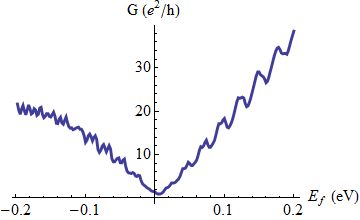
\includegraphics[scale=0.5]{images/exp-a-4}}
				\caption{Theoretical model.}
			\end{subfigure}
			\hspace{1cm}
			\begin{subfigure}{0.45\textwidth}
				\centerline{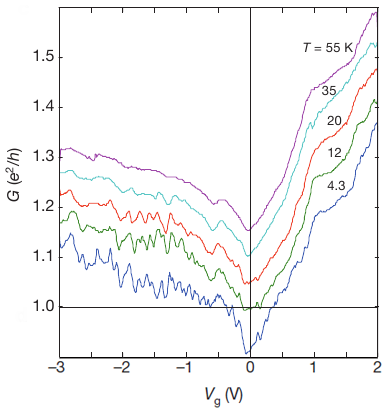
\includegraphics[scale=0.5]{images/exp-pa-4}}
				\caption{Experimental result from \cite{b19}.}
			\end{subfigure}
			\caption{Comparison of theoretical model for infinite graphene sheet against the experimental data for epitaxial graphene nanoribbons from \cite{b19}. The theoretical model here uses $V_{sd}=10$ mV, $T=20$ K, $V_{b}=0.9$ eV, $d=100$ nm, $m_{b}=0.6$ eV and an inverted gate dependence on $E_{f}$.}
			\label{exp-pa-4}
		\end{figure}

		Graphene nanoribbons (GNRs) that were epitaxially grown on silicon carbide have been shown to act as single channel, room temperature ballistic conductors  \cite{b19}. GNRs with a width of 40 nm were tested using a four point contact method. A 20 nm top gate made from Al$_{2}$O$_{3}$ coated with aluminium allowed the Fermi level of the system to be adjusted. These GNRs showed a large asymmetry with respect to gate voltage caused by np/pn doping and the presence of a semiconducting gap. The experimental results from the first of these devices is shown in Figure \ref{exp-pa-4} (b) with the theoretical results in Figure \ref{exp-pa-4} (a). To replicate the sharp changes in conductance at $E_{f}=0$ the dependence on gate voltage was flipped, then by introducing a high potential barrier, with a large energy gap in the barrier region the asymmetry of the experimental result was simulated.

		\begin{figure}[h]
			\begin{subfigure}{0.45\textwidth}
				\centerline{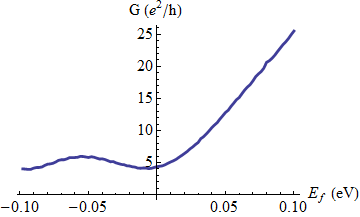
\includegraphics[scale=0.5]{images/exp-a-1}}
				\caption{Theoretical model.}
			\end{subfigure}
			\hspace{1cm}
			\begin{subfigure}{0.45\textwidth}
				\centerline{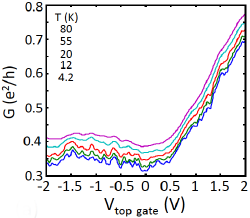
\includegraphics[scale=0.7]{images/exp-pa-1}}
				\caption{Experimental result from \cite{b19}.}
			\end{subfigure}
			\caption{Comparison of theoretical model for infinite graphene sheet against the experimental data for epitaxial graphene nanoribbons  from \cite{b19}[Supplementry Information]. The theoretical model here uses $V_{sd}=70$ mV, $T=55$ K, $V_{b}=0.1$ eV, $d=100$ nm, and a shifted $E_{f}$ of $+0.07$ eV.}
			\label{exp-pa-1}
		\end{figure}

		Alternate results in \cite{b19}[Supplementry Information] shown in Figure \ref{exp-pa-1}, were best modelled theoretically by a potential barrier with height $0.1$ eV and a shifted Fermi-energy of $+0.11$ eV. The smooth dependence of conductance on Fermi level implies a small barrier region was needed to replicate the experimental results; a small shift in Fermi level was then required to ensure the minima in conductance appeared at $E_{f}=0$ eV.

		\begin{figure}[h]
			\begin{subfigure}{0.45\textwidth}
				\centerline{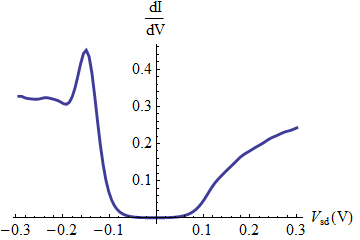
\includegraphics[scale=0.5]{images/exp-a-2}}
				\caption{Theoretical model.}
			\end{subfigure}
			\hspace{1cm}
			\begin{subfigure}{0.45\textwidth}
				\centerline{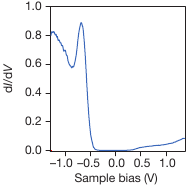
\includegraphics[scale=0.8]{images/exp-pa-2}}
				\caption{Experimental result from \cite{b19}.}
			\end{subfigure}
			\caption{Comparison of theoretical model for infinite graphene sheet against the experimental data for epitaxial graphene nanoribbons from \cite{b19}. The theoretical model here uses $V_{sd}=70$ mV, $T=55$ K, $V_{b}=0.1$ eV, $d=50$ nm, $m_{b}=0.06$ eV and a shifted $E_{f}$ of $+0.11$ eV.}
			\label{exp-pa-2}
		\end{figure}

		The differential conductance in Figure \ref{exp-pa-2} (b) from \cite{b19} shows very different results from the previous two cases; however, these results can be replicated using a theoretical model without the graphene density of states which is shown in Figure \ref{exp-pa-2} (a). With the linear dependence removed, a barrier with height $V_{b}=0.2$ eV and an energy gap of $m_{b}=0.1$ eV recreates the conductance peaks and zero conductance region.

		The use of a large potential barrier with an energy gap agrees with the analysis in \cite{b19}, where it is stated that the asymmery in results is caused by np/pn junctions and that n$\neq$0 subbands experience an energy gap. The theoretical model here does not show a strong temperature dependence. This is possibly due to the experimental results experiencing electronic heating not considered in the theoretical model.

		\begin{figure}[h]
			\begin{subfigure}{0.45\textwidth}
				\centerline{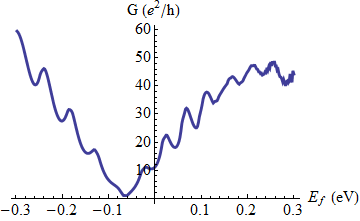
\includegraphics[scale=0.5]{images/exp-b-1}}
				\caption{Theoretical model.}
			\end{subfigure}
			\hspace{1cm}
			\begin{subfigure}{0.45\textwidth}
				\centerline{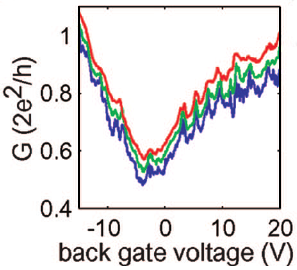
\includegraphics[scale=0.6]{images/exp-pb-1}}
				\caption{Experimental result from \cite{b20}.}
			\end{subfigure}
			\caption{Comparison of theoretical model for infinite graphene sheet against the experimental data for graphene nanoribbons pattered by plasma etching through a PMMA mask on a graphene flake from \cite{b20}. The theoretical model here uses $V_{sd}=10$ mV, $T=20$ K, $V_{b}=0.7$ eV, $m_{b}=0.2$ eV , $d=60$ nm and a shifted $E_{f}$ of $+0.06$ eV.}
			\label{exp-pb-1}
		\end{figure}

		The two probe measurements of 35 nm wide GNRs pattered by plasma etching through a PMMA (polymethyl methacrylate) mask on a graphene flake also show a large scale gap, with Fabry-P\'{e}rot resonances occuring in the graphene between the contacts and the constriction region when testing for the presence of a quantum dot \cite{b20}. Similarly to Figure \ref{exp-pa-4} the asymmetry in Figure \ref{exp-pb-1} can be recreated with a high potential barrier. The regular oscillations in conductance appear with low source-drain voltages and thin barrier regions. The location of the minimum in conductance implies that there is some shift in Fermi level which can be seen in Figure \ref{exp-pb-1}. The oscillations shown in Figure \ref{exp-pb-1} (a) are caused by Fabry-P\'{e}rot resonances within a single potential barrier in the theoretical model. This produces similar resonances to those caused in the graphene between the contacts and the constriction.

		\begin{figure}[h]
			\begin{subfigure}{0.45\textwidth}
				\centerline{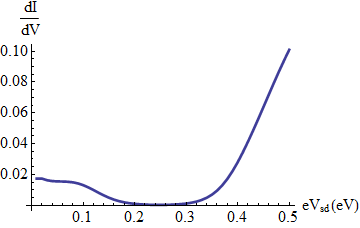
\includegraphics[scale=0.5]{images/exp-c-1}}
				\caption{Theoretical model.}
			\end{subfigure}
			\hspace{1cm}
			\begin{subfigure}{0.45\textwidth}
				\centerline{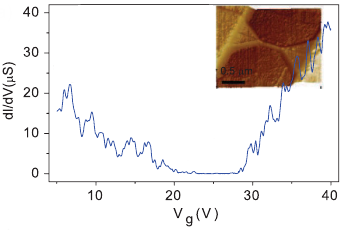
\includegraphics[scale=0.7]{images/exp-pc-1}}
				\caption{Experimental result from \cite{b21}.}
			\end{subfigure}
			\caption{Comparison of theoretical model for infinite graphene sheet against the experimental data for lithographically fabricated graphene nanoribbons from \cite{b21}. The theoretical model here uses $eV_{sd}=10$ mV, $T=300$ K, $V_{b}=0.25$ eV, $d=100$ nm and $m_{b}=0.12$ eV.}
			\label{exp-pc-1}
		\end{figure}

		The differential conductance of lithographically fabricated graphene nanoribbons studied in \cite{b21} is shown in Figure \ref{exp-pc-1} (b). The graphene nanoribbon here is placed on a highly doped silicon substrate with a 285 nm SiO$_{2}$ gate dielectric. These graphene nanoribbons show clear signs of an energy gap. The theroretical model in Figure \ref{exp-pc-1} (a) was created using a potential barrier with a height $V_{b}=0.25$ eV and an energy gap $m_{b}=0.12$ eV.

		\begin{figure}[h]
			\begin{subfigure}{0.45\textwidth}
				\centerline{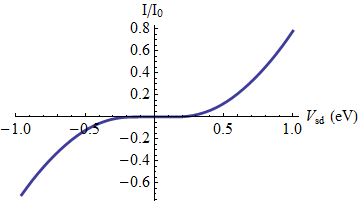
\includegraphics[scale=0.5]{images/exp-c-2}}
				\caption{Theoretical model.}
			\end{subfigure}
			\hspace{1cm}
			\begin{subfigure}{0.45\textwidth}
				\centerline{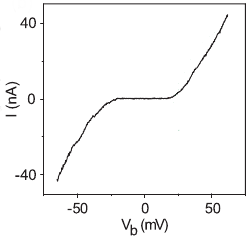
\includegraphics[scale=0.7]{images/exp-pc-2}}
				\caption{Experimental result from \cite{b21}.}
			\end{subfigure}
			\caption{Comparison of theoretical model for infinite graphene sheet against the experimental data for lithographically fabricated graphene nanoribbons from \cite{b21}. The theoretical model here uses $T=300$ K, $V_{b}=0$ eV, $d=100$ nm and $m_{b}=0.2$ eV.}
			\label{exp-pc-2}
		\end{figure}

		The current against source-drain voltage of these samples is shown in Figure \ref{exp-pc-2}. This result resembles charge carriers entering a region with an energy gap $m_{b}=0.2$ eV. The analysis in \cite{b21} states that the transport in the considered disordered system is dominated by hopping through localised states. The theoretical model with a potential barrier does include localised states and the comparison in Figure \ref{exp-pc-1} and Figure \ref{exp-pc-2} shows there are many similarities in results. Due to the disordered system diffusive transport is present. However, for the nano-scale system considered there is a high possibiliy that even in the presence of disorder there is some contribution from ballistic transport. The ballistic part of transport may explain the similarities in the shapes of the IV and conductance curves, while the additional disorder in the experimental data allows for the greatly reduced values of current.

		\begin{figure}[h]
			\begin{subfigure}{0.45\textwidth}
				\centerline{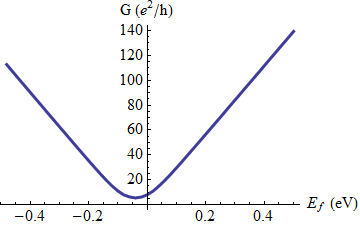
\includegraphics[scale=0.5]{images/exp-d-1}}
				\caption{Theoretical model.}
			\end{subfigure}
			\hspace{1cm}
			\begin{subfigure}{0.45\textwidth}
				\centerline{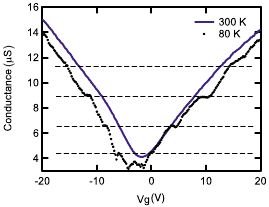
\includegraphics[scale=0.8]{images/exp-pd-1}}
				\caption{Experimental result from \cite{b22}.}
			\end{subfigure}
			\caption{Comparison of theoretical model for infinite graphene sheet against the experimental data for mechanically exfoliated graphene nanoribbons from \cite{b22}. The theoretical model here uses $T=300$ K, $V_{sd}=10$ mV, a Fermi energy shift of $+0.06$ eV and $V_{b}=0.05$ eV.}
			\label{exp-pd-1}
		\end{figure}
		
		In \cite{b22} a graphene nanoribbon is fabricated from mechanically exfoliated graphene. This is placed on p-doped silicon covered with 300 nm thick SiO$_{2}$, then placed between palladium contacts. The mostly linear dependence of conductance on the Fermi energy can be seen in Figure \ref{exp-pd-1} (b) and implies no scattering region between the two contacts, however, at low temperatures the results do show signs of a small scattering region. As the condunctance minimum is not at $E_{f}=0$ eV a shift of $+0.2$ eV has been used for the theoretical model in Figure \ref{exp-pd-1} (a).  The anaylsis in \cite{b22} states that the asymmetry of the conductance is likely caused by some form of gate oxide hysteresis. For one sample a gate voltage of 20 V is used, it is stated that this corresponds to a shift in the Fermi level of approximately 0.26 eV, indicating that there is a large contact resistance present that was not accounted for in the theoretical model.

		While many of the experimental results resemble the theoretical model, many features vary by orders of magnitude. The sample bias for nearly all experimental results is vastly greater then the predicted change in Fermi energy. This is possibly due to some form of contact resistance; the voltage applied to the gate region is not perfectly affecting the Fermi level of the graphene. It would therefore require much larger external voltages to change the Fermi level of the sample. This contact resistance will also change how the current is carried through a sample of graphene; if a voltage probe is placed in an obtrusive manor it may act as an additional scattering region, reducing the flow of current. The observed effect of temperature is greater than predicted, as described in \cite{b19} an experimental sample will experience some heating when a current is passed through it. It is therefore possible that in order to achieve similar temperature dependences a larger temperature difference will be required.

		The theoretical results in Figure \ref{exp-pa-4} and Figure \ref{exp-pb-1} show clear resonances at regular intervals of energy. As these results both use potential barrier regions with large heights, these resoances can be described by the Fabry-P\'{e}rot resonance condition with large potentials.
			\begin{equation}
				E=\pm \frac{\hbar v_{f}n \pi}{d}
			\end{equation}
		The corresponding experimental results also show regular peaks in the conductance plots, it is possible that resonances are contributing to these conductance peaks.

%\end{document}